\documentclass[english,11pt]{beamer}

\DeclareMathOperator{\Cov}{Cov}
\DeclareMathOperator{\Var}{Var}
\DeclareMathOperator{\E}{\mathbb{E}}
\DeclareMathOperator{\Proba}{\mathbb{P}}

\newcommand{\Covb}[2]{\ensuremath{\Cov\!\left[#1,#2\right]}}
\newcommand{\Eb}[1]{\ensuremath{\E\!\left[#1\right]}}
\newcommand{\Pb}[1]{\ensuremath{\Proba\!\left[#1\right]}}
\newcommand{\Varb}[1]{\ensuremath{\Var\!\left[#1\right]}}

% norm
\newcommand{\norm}[1]{\| #1 \|}

\newcommand{\indep}{\rotatebox[origin=c]{90}{$\models$}}





\usepackage{mathptmx,amsmath,amssymb,graphicx,bibentry,bbm,babel,ragged2e}

\makeatletter

\newcommand{\noun}[1]{\textsc{#1}}
\newcommand{\jitem}[1]{\item \begin{justify} #1 \end{justify} \vfill{}}
\newcommand{\sframe}[2]{\frame{\frametitle{#1} #2}}

\newenvironment{centercolumns}{\begin{columns}[c]}{\end{columns}}
%\newenvironment{jitem}{\begin{justify}\begin{itemize}}{\end{itemize}\end{justify}}

\usetheme{Warsaw}
\setbeamertemplate{footline}[text line]{}
\setbeamercolor{structure}{fg=purple!50!blue, bg=purple!50!blue}

\setbeamersize{text margin left=15pt,text margin right=15pt}

\setbeamercovered{transparent}


\@ifundefined{showcaptionsetup}{}{%
 \PassOptionsToPackage{caption=false}{subfig}}
\usepackage{subfig}

\usepackage[utf8]{inputenc}
\usepackage[T1]{fontenc}



\makeatother

\begin{document}


\title{A Discrepancy-based Framework to Compare Robustness between Multi-Attribute Evaluations}

\author{J.~Raimbault$^{1,2}$\\
\texttt{juste.raimbault@parisgeo.cnrs.fr}
}


\institute{$^{1}$UMR CNRS 8504 G{\'e}ographie-cit{\'e}s\\
$^{2}$UMR-T IFSTTAR 9403 LVMT\\
}


\date{CSDM 2016 - Paris\\\smallskip
14th December 2016
}

\frame{\maketitle}


%%%
% Abstract

%Multi-objective evaluation is a necessary aspect when managing complex systems, as the intrinsic complexity of a system is generally closely linked to the potential number of optimization objectives. However, an evaluation makes no sense without its robustness being given (in the sense of its reliability). Statistical robustness computation methods are highly dependent of underlying statistical models. We propose a formulation of a model-independent framework in the case of integrated aggregated indicators (multi-attribute evaluation), that allows to define a relative measure of robustness taking into account data structure and indicator values. We implement and apply it to a synthetic case of urban systems based on Paris districts geography, and to real data for evaluation of income segregation for Greater Paris metropolitan area. First numerical results show the potentialities of this new method. Furthermore, its relative independence to system type and model may position it as an alternative to classical statistical robustness methods.
%\keywords{Multi-attribute Evaluation, Model-Independent Robustness, Urban System, Discrepancy}




%%%%%%%%%%%%%%%%%
\section{Introduction}
%%%%%%%%%%%%%%%%%


\sframe{Complex systems}{

% introduction with pictures/anecdote

}



\sframe{Multi-attribute Evaluation in Complex Socio-technical Systems}{

\justify

\textit{Systematic multi-objective nature of problems in design of Complex Industrial Systems~\cite{marler2004survey} and in the study of Complex Natural Systems~\cite{newman2011complex}}

\medskip

$\rightarrow$ 

\medskip

$\rightarrow$ Territorial systems as typical examples : e.g. sustainable urban design~\cite{souami2012ecoquartiers}, multi-criteria decision-making for transportation infrastructures~\cite{bavoux2005geographie}



}


\sframe{Robustness of Evaluations}{

\justify

.


}


\sframe{Towards a Generic Robustness Framework}{

\justify

\textbf{Research Objective : } \textit{Investigate a generic data-driven approach to Robustness in Multi-attribute evaluations of Complex Socio-Technical Systems}

% put rationales here

\bigskip

$\rightarrow$ 
\medskip

$\rightarrow$ 

}


%%%%%%%%%%%%%%%%%
\section{Framework Description}
%%%%%%%%%%%%%%%%%



\sframe{Theoretical Framing}{

% here theory is in the sense of thematic theory



}


\sframe{Assumptions}{
\justify

% assumptions done

\textbf{Objectives as Spatial Integrals}


\medskip

\textbf{Linearly Aggregated Objectives}


}



\sframe{Formal Description (I)}{


Territorial Systems $S_{i}=(\mathbf{X}_{i},\mathbf{Y}_{i})\in\mathcal{X}_{i}\times\mathcal{Y}_{i}$ with $\mathcal{X}_{i}=\prod_{k}\mathcal{X}_{i,k}$ 


\[
(\mathcal{X},\mathcal{Y}) \underset{def}{=} \left(\prod\tilde{\mathcal{X}}_{c}\right)\times\left(\prod\tilde{\mathcal{Y}}_{c}\right) = \left(\prod_{\mathcal{X}_{i,k}\in\mathcal{D}_{\mathcal{X}}}\mathbb{R}^{p_{i,k}^{X}}\right)\times\left(\prod_{\mathcal{Y}_{i,k}\in\mathcal{D}_{\mathcal{Y}}}\mathbb{R}^{p_{i,k}^{Y}}\right)
\]



Objectives : $H_{c}$ space of real-valued functions on $(\tilde{\mathcal{X}}_{c},\tilde{\mathcal{Y}}_{c})$, such that for all $h\in H_{c}$ :
\begin{enumerate}
\item $h$ is ``enough'' regular (tempered distributions e.g.)
\item $q_c=\int_{(\tilde{\mathcal{X}}_{c},\tilde{\mathcal{Y}}_{c})}h$ is a function describing the ``urban fact'' (the indicator in itself)
\end{enumerate}


}




\sframe{Formal Description (II)}{

Integral approximation theorem gives upper bound on error, linked to data discrepancy~\cite{niederreiter1972discrepancy}\cite{varet2010developpement}

\[
\left\Vert \int h_{c}-\frac{1}{n_{i,c}}\sum_{l}h_{c}(\vec{X}_{i,c,l})\right\Vert \leq K\cdot\left|\left|\left|h_{c}\right|\right|\right|\cdot D_{i,c}
\]

which propagates to the linear aggregation

\[
\left\Vert \int\sum w_{i,c}h_{c}-\frac{1}{n_{i,c}}\sum_{l}w_{i,c}h_{c}(\vec{X}_{i,c,l})\right\Vert \leq K\sum_{c}\left|w_{i,c}\right|\left|\left|\left|h_{c}\right|\right|\right|\cdot D_{i,c}
\]


}


\sframe{Formal Description (III)}{

A relative \textit{Robustness Ratio} can thus be defined between two evaluations :

\begin{equation}
R_{i,i'}=\frac{\sum_{c}w_{i,c}\cdot D_{i,c}}{\sum_{c}w_{i',c}\cdot D_{i',c}}
\end{equation}


}





%%%%%%%%%%%%%%%%%
\section{Results}
%%%%%%%%%%%%%%%%%




\sframe{Implementation on Synthetic Data}{

% summary, data description, main result (summary of table)

}

\sframe{Metropolitan Segregation}{

% indicators, data

Metropolitan Segregation on Ile-de-France, Insee income data (2011)

\medskip

\textbf{Indicators : }

\begin{itemize}
\item Spatial autocorrelation Moran index, defined as weighted normalized covariance of median income by $\rho = \frac{N}{\sum_{ij}w_{ij}}\cdot \frac{\sum_{ij}w_{ij}\left(X_i - \bar{X}\right)\left(X_j - \bar{X}\right)}{\sum_i \left(X_i - \bar{X}\right)^2}$
\item Dissimilarity index (close to Moran but integrating local dissimilarities rather than correlations), given by $d =  \frac{1}{\sum_{ij}w_{ij}} \sum_{ij} w_{ij} \left|\tilde{X}_i - \tilde{X}_j\right|$\\ with $\tilde{X}_i = \frac{X_i - \min(X_k)}{\max(X_k) - \min(X_k)}$
\item Complementary of the entropy of income distribution that is a way to capture global inequalities $\varepsilon = 1 + \frac{1}{\log(N)} \sum_i \frac{X_i}{\sum_k X_k} \cdot \log\left(\frac{X_i}{\sum_k X_k}\right)$
\end{itemize}

}

\sframe{Metropolitan Segregation}{

% segreg maps

\textit{Example of Segregation maps}

\medskip

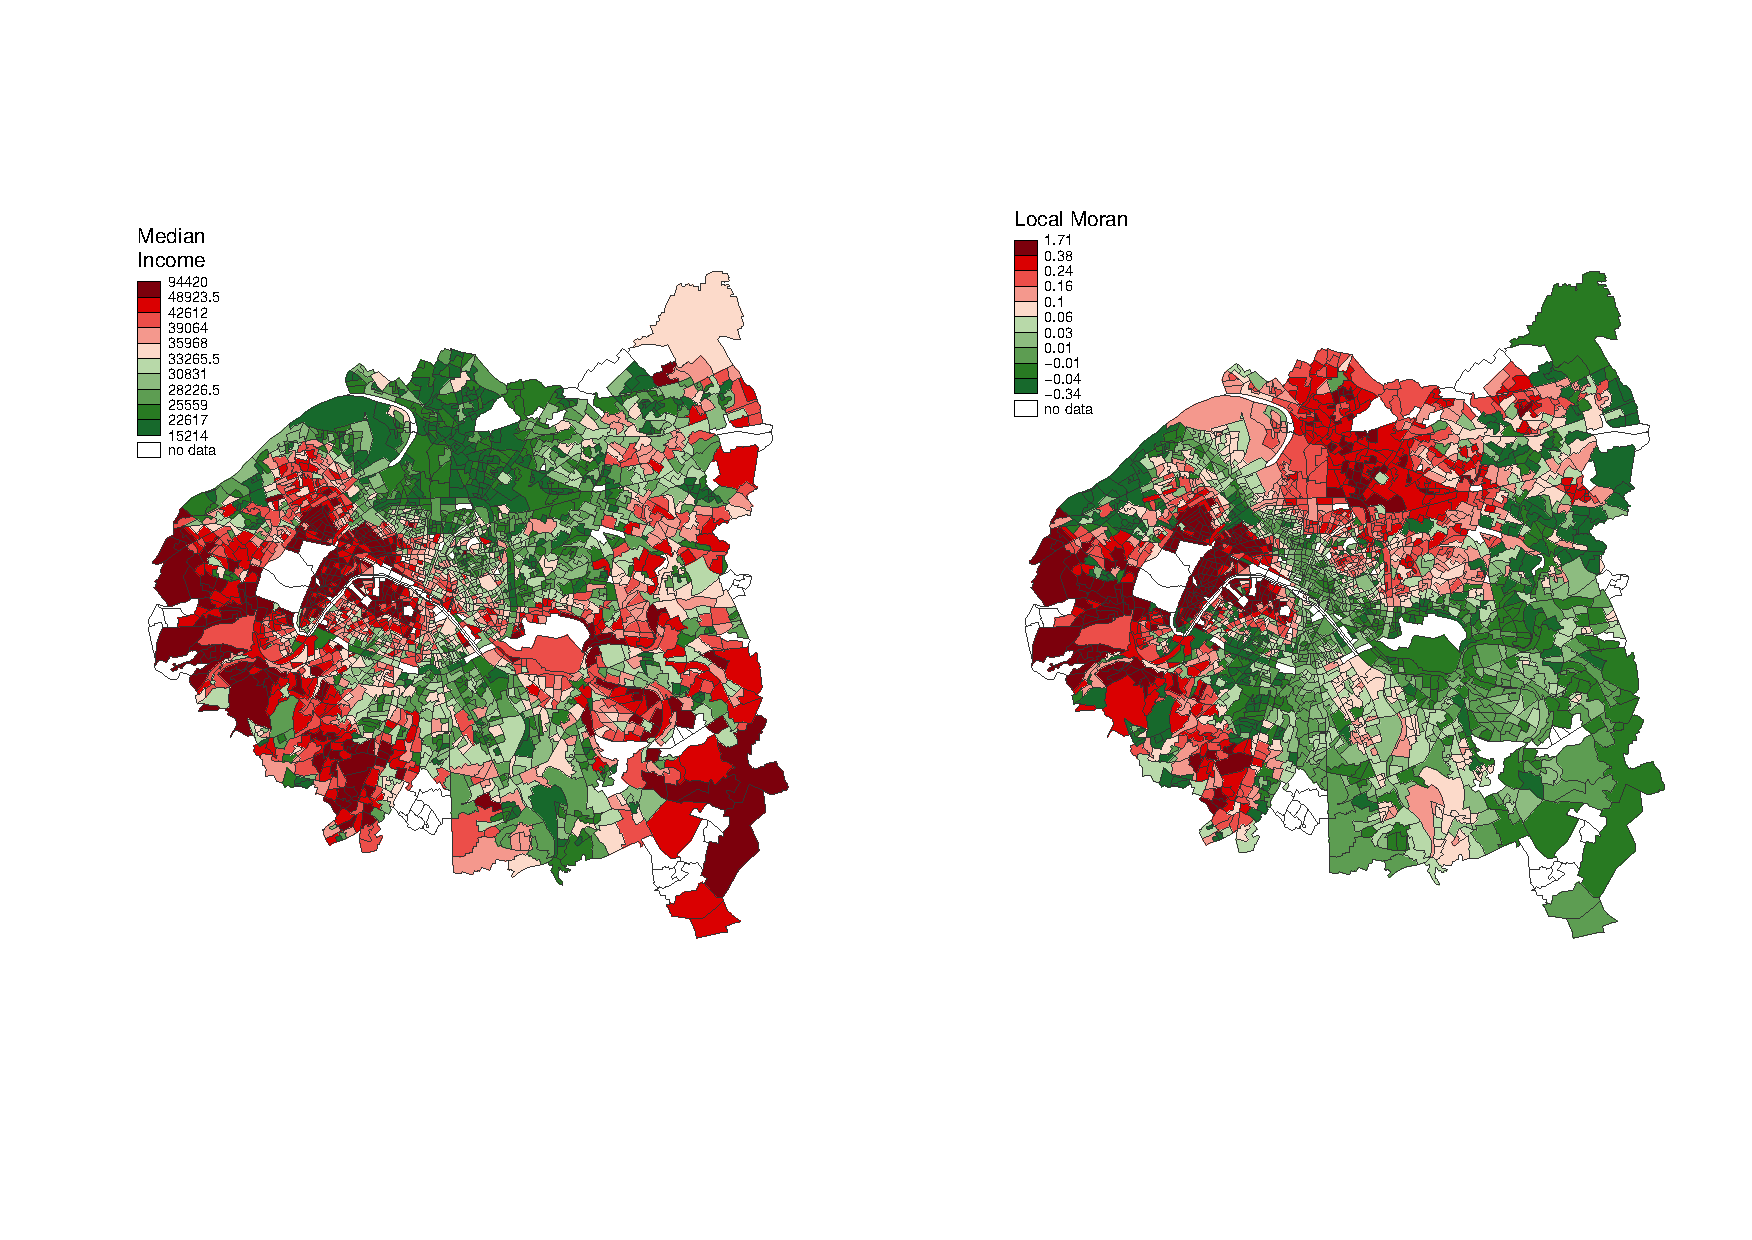
\includegraphics[width=\textwidth]{figures/grandParis_income_moran}


}


\sframe{Metropolitan Segregation}{

% missing data
\textit{Framework Application : sensitivity to missing data}

\medskip

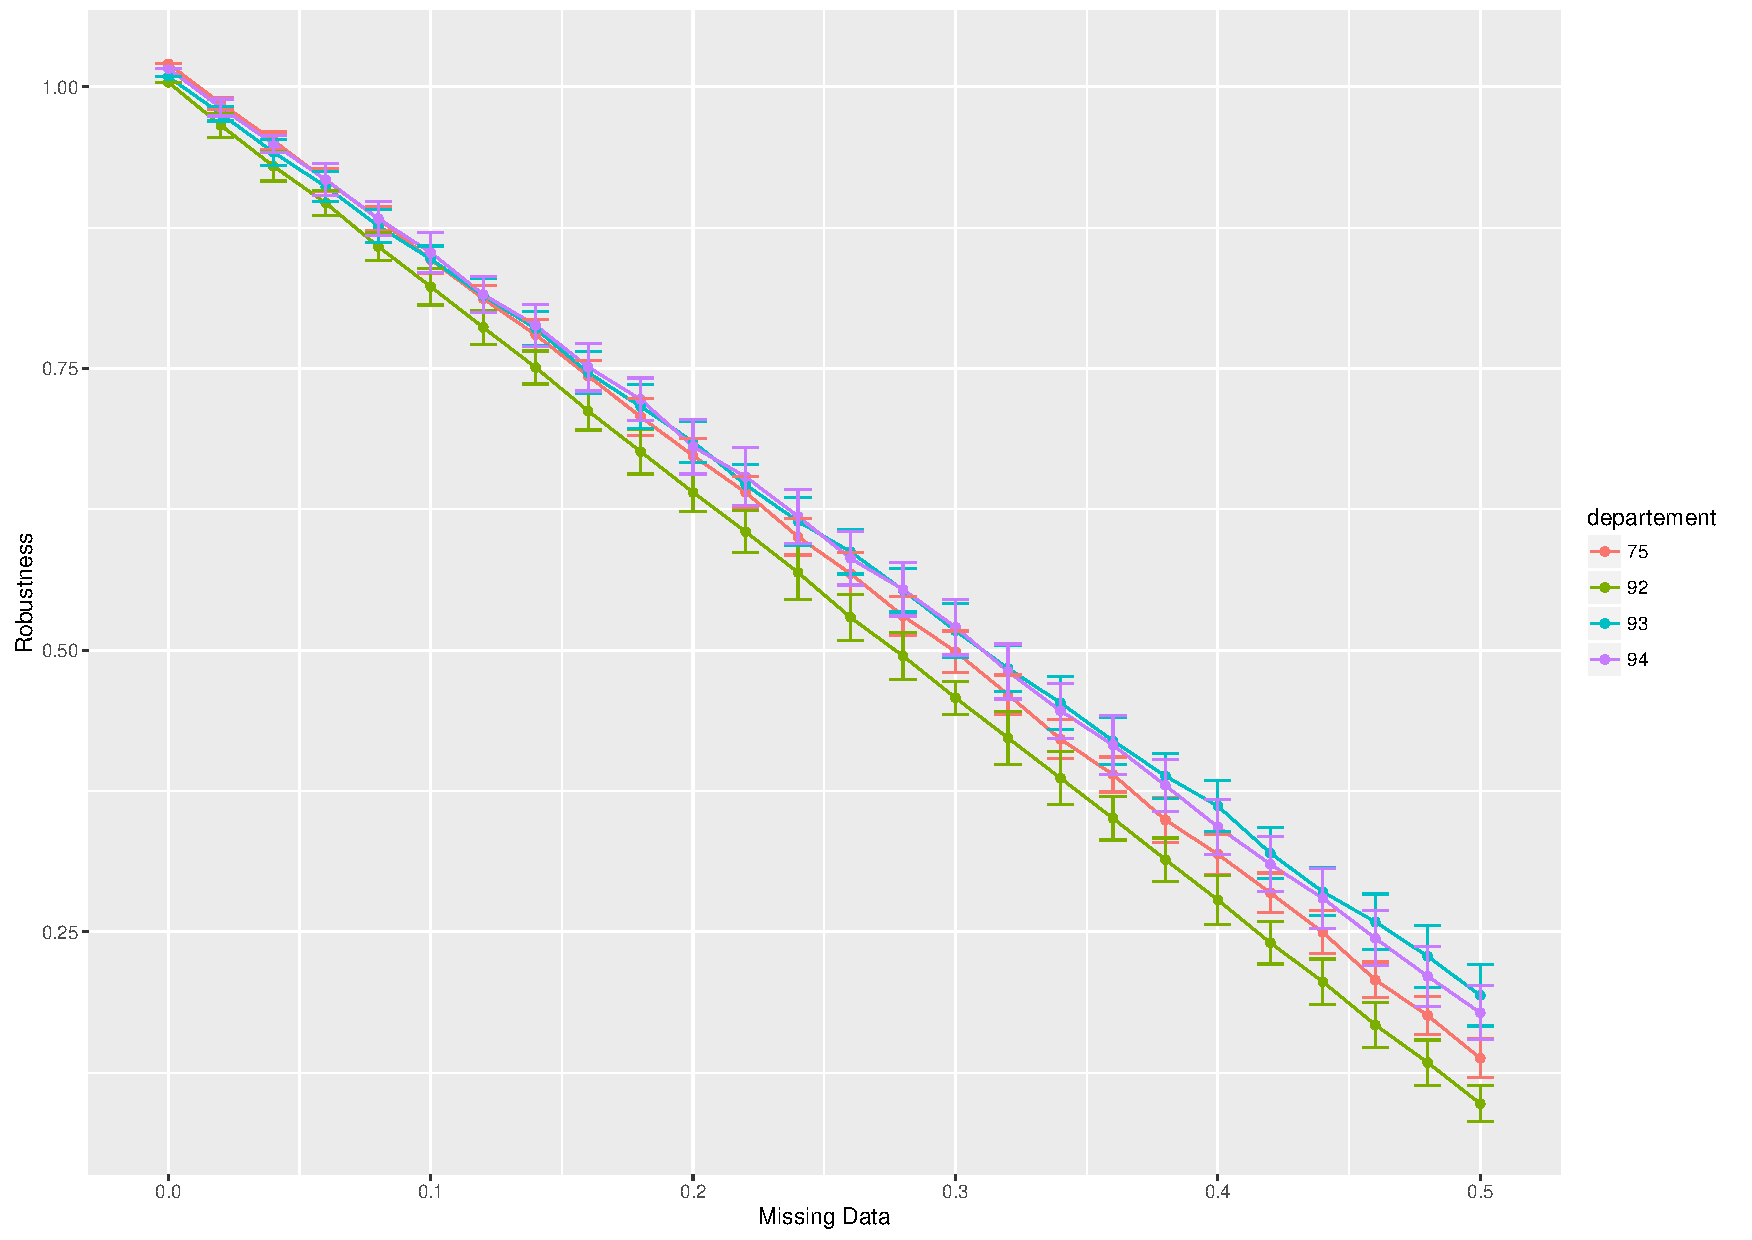
\includegraphics[width=0.45\textwidth]{figures/alldeps_rob_renormindics}

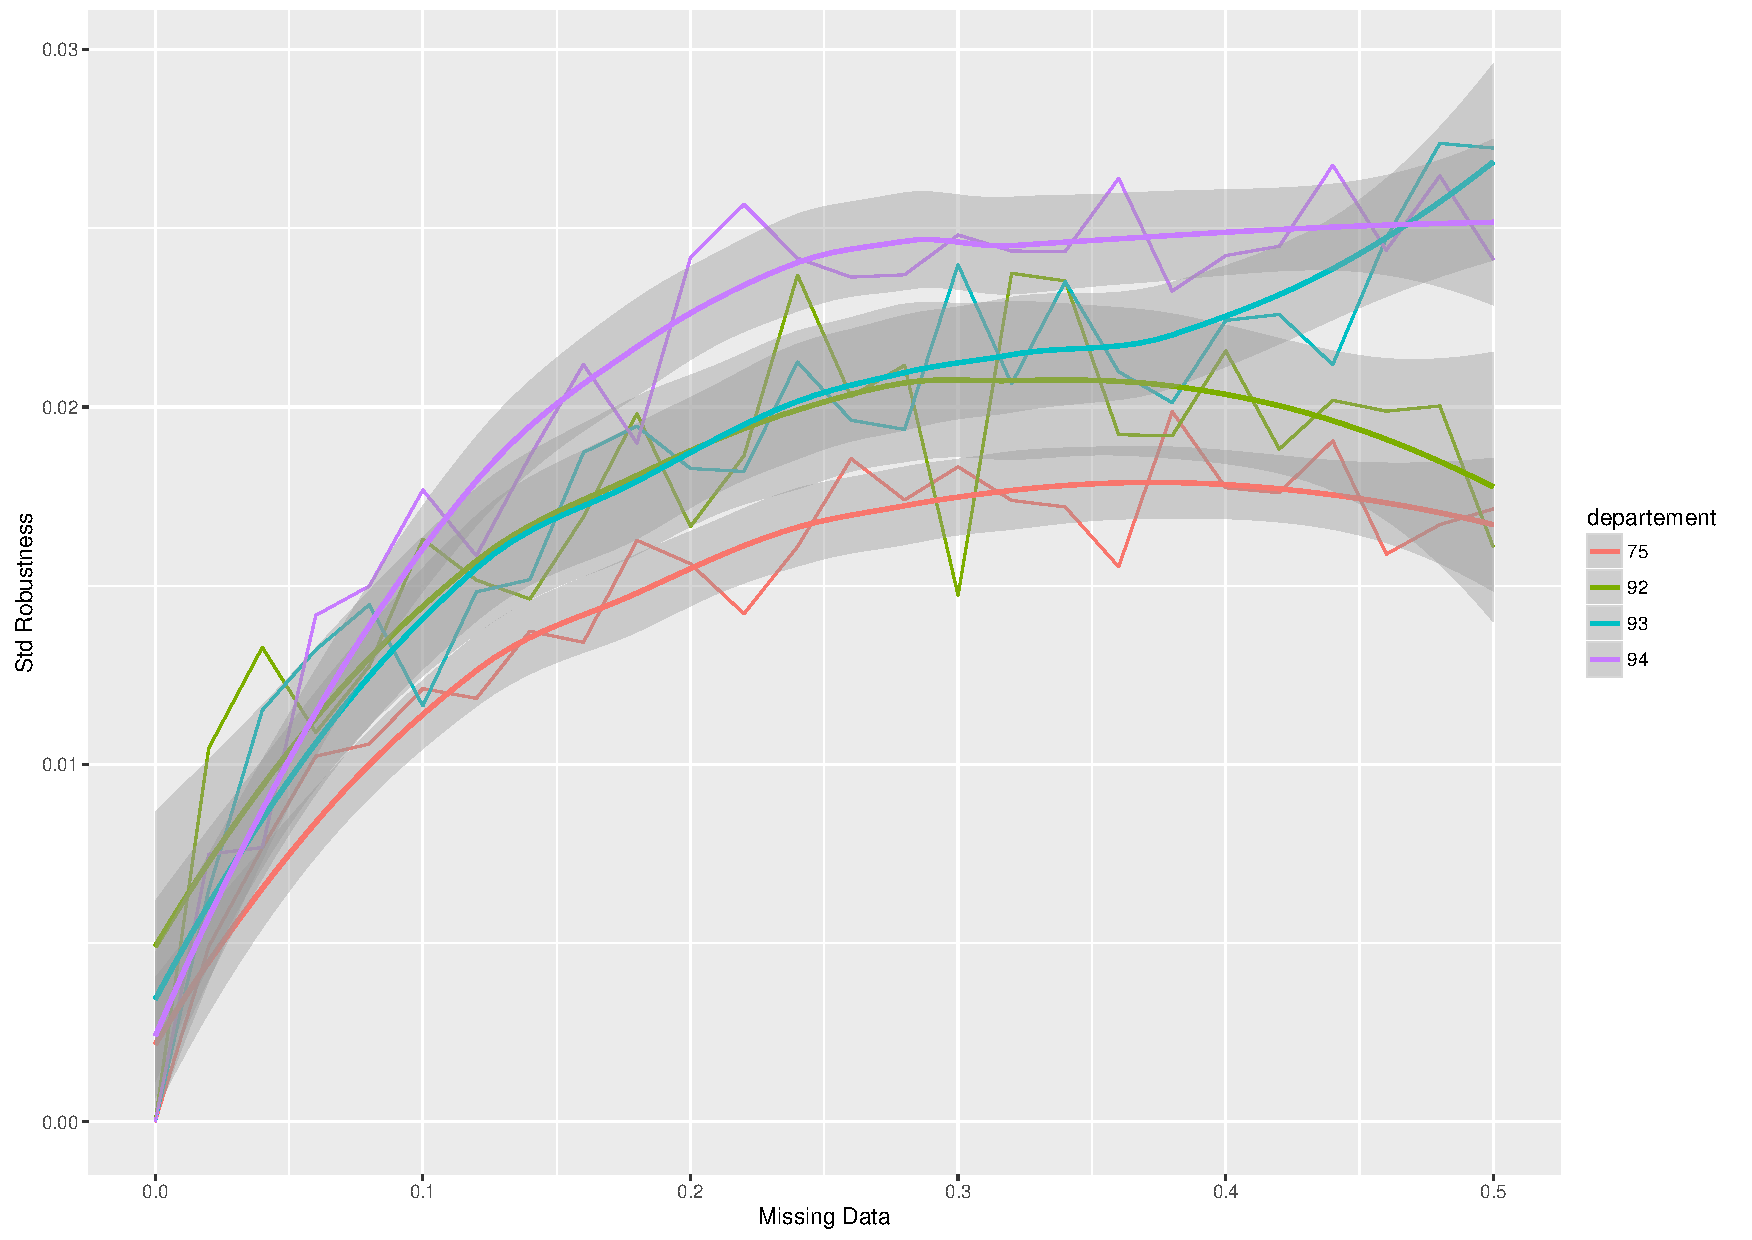
\includegraphics[width=0.45\textwidth]{figures/alldeps_robsd_renormindics}

% interpretation : different regimes.


}




%%%%%%%%%%%%%%%%%
\section{Discussion}
%%%%%%%%%%%%%%%%%


\sframe{Applicability}{

\justify

$\rightarrow$ Application to decision-making procedures : adding robustness as a dimension ?

\medskip

$\rightarrow$ Availability of raw data

\medskip

$\rightarrow$ Assumptions validity ranges : some indicators may difficultly be viewed as spatial integrals (as some accessibility measures~\cite{kwan1998space}

}




\sframe{Further Developments}{

\justify

$\rightarrow$ Application to existing open frameworks (e.g. \cite{tivadar2014oasis})


\medskip

$\rightarrow$ More general formulation, first to non-linear aggregation (e.g. for Lipschitzian functions~\cite{dragomir1999ostrowski})

}



\sframe{Conclusion}{

$\rightarrow$ 

\medskip


\bigskip
\bigskip
\bigskip


\footnotesize{ - All code available at \texttt{https://github.com/JusteRaimbault/RobustnessDiscrepancy}

\medskip

 - Paper preprint available at \texttt{http://arxiv.org/abs/}
}

}






%%%%%%%%%%%%%%%%%%%%%
\begin{frame}[allowframebreaks]
\frametitle{References}
\bibliographystyle{apalike}
\bibliography{/Users/Juste/Documents/ComplexSystems/CityNetwork/Biblio/Bibtex/CityNetwork,biblio}
\end{frame}
%%%%%%%%%%%%%%%%%%%%%%%%%%%%












\end{document}







